\documentclass[14pt]{extbook}
\usepackage{multicol, enumerate, enumitem, hyperref, color, soul, setspace, parskip, fancyhdr} %General Packages
\usepackage{amssymb, amsthm, amsmath, latexsym, units, mathtools} %Math Packages
\everymath{\displaystyle} %All math in Display Style
% Packages with additional options
\usepackage[headsep=0.5cm,headheight=12pt, left=1 in,right= 1 in,top= 1 in,bottom= 1 in]{geometry}
\usepackage[usenames,dvipsnames]{xcolor}
\usepackage{dashrule}  % Package to use the command below to create lines between items
\newcommand{\litem}[1]{\item#1\hspace*{-1cm}\rule{\textwidth}{0.4pt}}
\pagestyle{fancy}
\lhead{Progress Quiz 9}
\chead{}
\rhead{Version C}
\lfoot{9541-5764}
\cfoot{}
\rfoot{Summer C 2021}
\begin{document}

\begin{enumerate}
\litem{
Solve the quadratic equation below. Then, choose the intervals that the solutions $x_1$ and $x_2$ belong to, with $x_1 \leq x_2$.\[ 25x^{2} -60 x + 36 = 0 \]\begin{enumerate}[label=\Alph*.]
\item \( x_1 \in [0.54, 0.61] \text{ and } x_2 \in [1.77, 2.78] \)
\item \( x_1 \in [0.17, 0.35] \text{ and } x_2 \in [4.56, 6.52] \)
\item \( x_1 \in [29.74, 30.37] \text{ and } x_2 \in [29.71, 30.04] \)
\item \( x_1 \in [0.76, 1.75] \text{ and } x_2 \in [1.01, 1.77] \)
\item \( x_1 \in [0.37, 0.55] \text{ and } x_2 \in [3.25, 4.59] \)

\end{enumerate} }
\litem{
Write the equation of the graph presented below in the form $f(x)=ax^2+bx+c$, assuming  $a=1$ or $a=-1$. Then, choose the intervals that $a, b,$ and $c$ belong to.
\begin{center}
    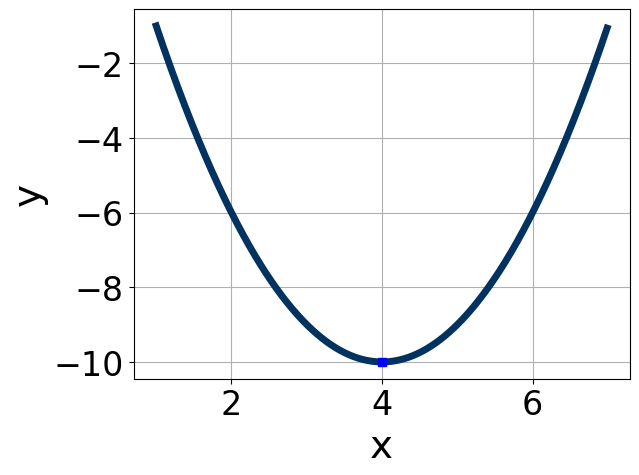
\includegraphics[width=0.5\textwidth]{../Figures/quadraticGraphToEquationC.png}
\end{center}
\begin{enumerate}[label=\Alph*.]
\item \( a \in [-1.8, -0.5], \hspace*{5mm} b \in [-10, -5], \text{ and } \hspace*{5mm} c \in [-26, -23] \)
\item \( a \in [0.7, 1.1], \hspace*{5mm} b \in [5, 11], \text{ and } \hspace*{5mm} c \in [6, 9] \)
\item \( a \in [-1.8, -0.5], \hspace*{5mm} b \in [5, 11], \text{ and } \hspace*{5mm} c \in [-26, -23] \)
\item \( a \in [0.7, 1.1], \hspace*{5mm} b \in [-10, -5], \text{ and } \hspace*{5mm} c \in [6, 9] \)
\item \( a \in [0.7, 1.1], \hspace*{5mm} b \in [5, 11], \text{ and } \hspace*{5mm} c \in [25, 27] \)

\end{enumerate} }
\litem{
Graph the equation below.\[ f(x) = -(x+1)^2 + 10 \]\begin{enumerate}[label=\Alph*.]
\begin{multicols}{2}\item 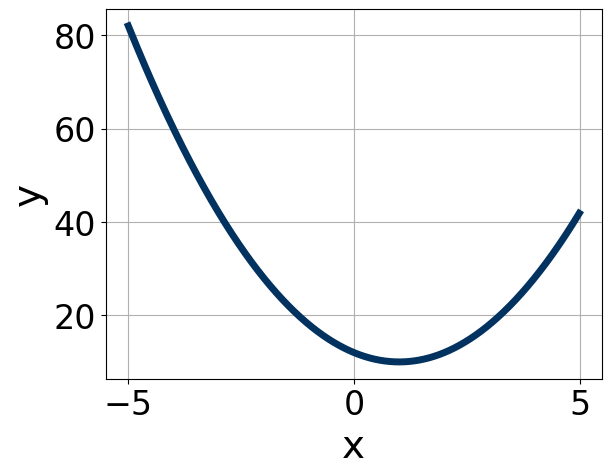
\includegraphics[width = 0.3\textwidth]{../Figures/quadraticEquationToGraphCopyAC.png}\item 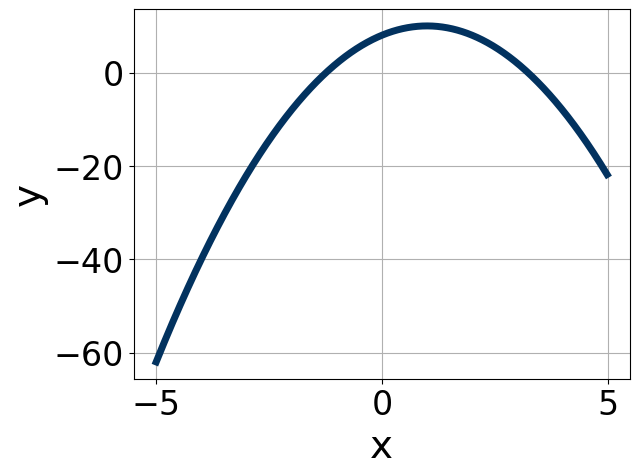
\includegraphics[width = 0.3\textwidth]{../Figures/quadraticEquationToGraphCopyBC.png}\item 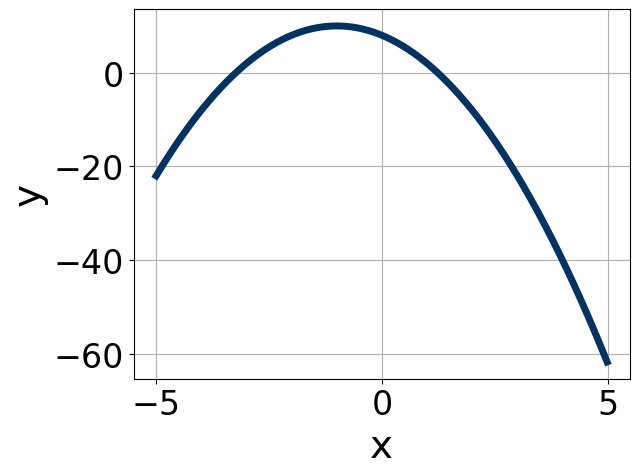
\includegraphics[width = 0.3\textwidth]{../Figures/quadraticEquationToGraphCopyCC.png}\item 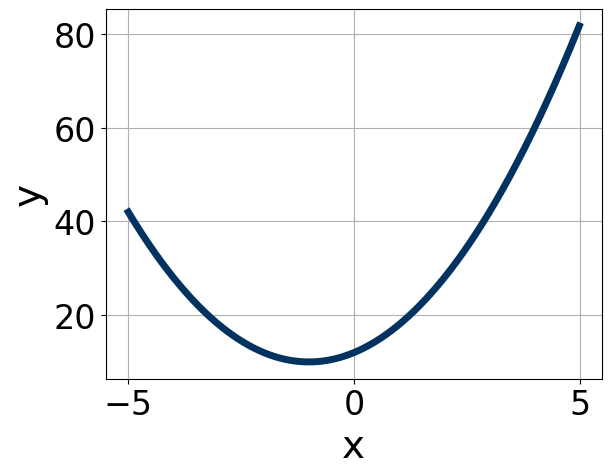
\includegraphics[width = 0.3\textwidth]{../Figures/quadraticEquationToGraphCopyDC.png}\end{multicols}\item None of the above.
\end{enumerate} }
\litem{
Graph the equation below.\[ f(x) = -(x+2)^2 + 11 \]\begin{enumerate}[label=\Alph*.]
\begin{multicols}{2}\item 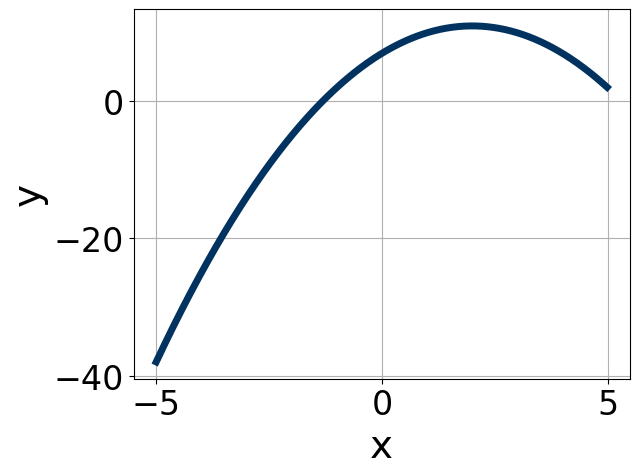
\includegraphics[width = 0.3\textwidth]{../Figures/quadraticEquationToGraphAC.png}\item 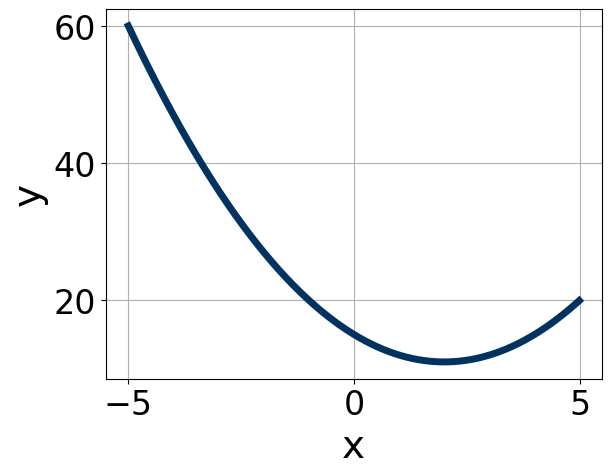
\includegraphics[width = 0.3\textwidth]{../Figures/quadraticEquationToGraphBC.png}\item 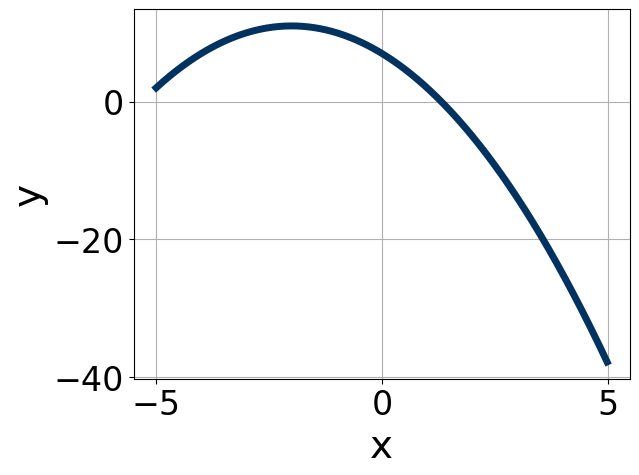
\includegraphics[width = 0.3\textwidth]{../Figures/quadraticEquationToGraphCC.png}\item 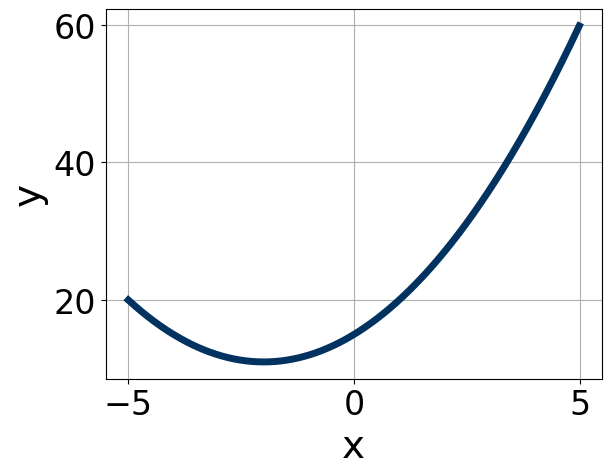
\includegraphics[width = 0.3\textwidth]{../Figures/quadraticEquationToGraphDC.png}\end{multicols}\item None of the above.
\end{enumerate} }
\litem{
Solve the quadratic equation below. Then, choose the intervals that the solutions $x_1$ and $x_2$ belong to, with $x_1 \leq x_2$.\[ 25x^{2} -60 x + 36 = 0 \]\begin{enumerate}[label=\Alph*.]
\item \( x_1 \in [0.07, 0.26] \text{ and } x_2 \in [5.1, 7.2] \)
\item \( x_1 \in [0.33, 0.56] \text{ and } x_2 \in [2.8, 4] \)
\item \( x_1 \in [0.93, 1.44] \text{ and } x_2 \in [0.9, 2] \)
\item \( x_1 \in [0.53, 0.83] \text{ and } x_2 \in [2.1, 2.8] \)
\item \( x_1 \in [29.93, 30.26] \text{ and } x_2 \in [29.6, 30.2] \)

\end{enumerate} }
\litem{
Solve the quadratic equation below. Then, choose the intervals that the solutions belong to, with $x_1 \leq x_2$ (if they exist).\[ -10x^{2} -7 x + 2 = 0 \]\begin{enumerate}[label=\Alph*.]
\item \( x_1 \in [-2.59, -2.04] \text{ and } x_2 \in [9.07, 10.05] \)
\item \( x_1 \in [-13.12, -11.38] \text{ and } x_2 \in [10.67, 11.15] \)
\item \( x_1 \in [-0.75, 0.18] \text{ and } x_2 \in [0.63, 1.43] \)
\item \( x_1 \in [-1.05, -0.78] \text{ and } x_2 \in [-0.47, 0.34] \)
\item \( \text{There are no Real solutions.} \)

\end{enumerate} }
\litem{
Write the equation of the graph presented below in the form $f(x)=ax^2+bx+c$, assuming  $a=1$ or $a=-1$. Then, choose the intervals that $a, b,$ and $c$ belong to.
\begin{center}
    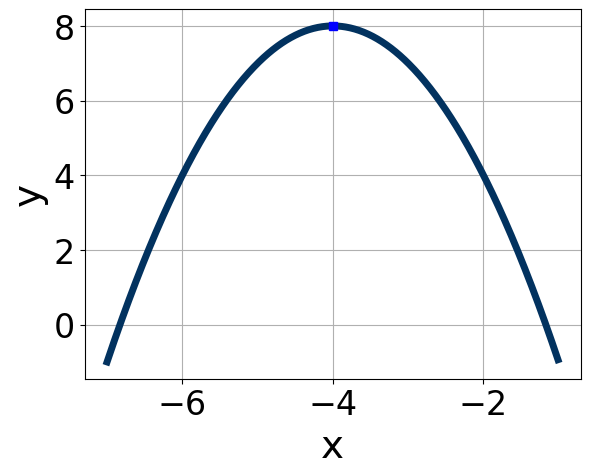
\includegraphics[width=0.5\textwidth]{../Figures/quadraticGraphToEquationCopyC.png}
\end{center}
\begin{enumerate}[label=\Alph*.]
\item \( a \in [-2, 0], \hspace*{5mm} b \in [5, 12], \text{ and } \hspace*{5mm} c \in [-9, -7] \)
\item \( a \in [-2, 0], \hspace*{5mm} b \in [-8, -7], \text{ and } \hspace*{5mm} c \in [-9, -7] \)
\item \( a \in [-2, 0], \hspace*{5mm} b \in [5, 12], \text{ and } \hspace*{5mm} c \in [-24, -18] \)
\item \( a \in [1, 2], \hspace*{5mm} b \in [-8, -7], \text{ and } \hspace*{5mm} c \in [21, 28] \)
\item \( a \in [1, 2], \hspace*{5mm} b \in [5, 12], \text{ and } \hspace*{5mm} c \in [21, 28] \)

\end{enumerate} }
\litem{
Factor the quadratic below. Then, choose the intervals that contain the constants in the form $(ax+b)(cx+d); b \leq d.$\[ 36x^{2} +37 x -10 \]\begin{enumerate}[label=\Alph*.]
\item \( a \in [2, 3.3], \hspace*{5mm} b \in [-4, 0], \hspace*{5mm} c \in [11.51, 12.51], \text{ and } \hspace*{5mm} d \in [5, 11] \)
\item \( a \in [14.6, 18.7], \hspace*{5mm} b \in [-4, 0], \hspace*{5mm} c \in [1.12, 2.35], \text{ and } \hspace*{5mm} d \in [5, 11] \)
\item \( a \in [6.4, 9.6], \hspace*{5mm} b \in [-4, 0], \hspace*{5mm} c \in [3.3, 4.64], \text{ and } \hspace*{5mm} d \in [5, 11] \)
\item \( a \in [-0.7, 2.2], \hspace*{5mm} b \in [-8, -4], \hspace*{5mm} c \in [0.62, 1.09], \text{ and } \hspace*{5mm} d \in [40, 50] \)
\item \( \text{None of the above.} \)

\end{enumerate} }
\litem{
Factor the quadratic below. Then, choose the intervals that contain the constants in the form $(ax+b)(cx+d); b \leq d.$\[ 54x^{2} -57 x + 10 \]\begin{enumerate}[label=\Alph*.]
\item \( a \in [16, 20], \hspace*{5mm} b \in [-8, -4], \hspace*{5mm} c \in [1.1, 3.8], \text{ and } \hspace*{5mm} d \in [-8, -1] \)
\item \( a \in [2, 4], \hspace*{5mm} b \in [-8, -4], \hspace*{5mm} c \in [15.3, 18.3], \text{ and } \hspace*{5mm} d \in [-8, -1] \)
\item \( a \in [-1, 2], \hspace*{5mm} b \in [-47, -41], \hspace*{5mm} c \in [-1.5, 1.3], \text{ and } \hspace*{5mm} d \in [-12, -9] \)
\item \( a \in [4, 8], \hspace*{5mm} b \in [-8, -4], \hspace*{5mm} c \in [6.7, 12.2], \text{ and } \hspace*{5mm} d \in [-8, -1] \)
\item \( \text{None of the above.} \)

\end{enumerate} }
\litem{
Solve the quadratic equation below. Then, choose the intervals that the solutions belong to, with $x_1 \leq x_2$ (if they exist).\[ 17x^{2} +9 x -3 = 0 \]\begin{enumerate}[label=\Alph*.]
\item \( x_1 \in [-17.47, -16.76] \text{ and } x_2 \in [16.34, 17.07] \)
\item \( x_1 \in [-0.3, 0.67] \text{ and } x_2 \in [0.59, 1.42] \)
\item \( x_1 \in [-13.31, -12.64] \text{ and } x_2 \in [3.72, 4.19] \)
\item \( x_1 \in [-0.82, -0.57] \text{ and } x_2 \in [-0.77, 0.32] \)
\item \( \text{There are no Real solutions.} \)

\end{enumerate} }
\end{enumerate}

\end{document}